\documentclass[conference]{IEEEtran}
\IEEEoverridecommandlockouts
% The preceding line is only needed to identify funding in the first footnote. If that is unneeded, please comment it out.
%Template version as of 6/27/2024

\usepackage{cite}
\usepackage{amsmath,amssymb,amsfonts}
\usepackage{algorithmic}
\usepackage{graphicx}
\usepackage{textcomp}
\usepackage{xcolor}
\usepackage{mathtools}
\usepackage{float}
\usepackage{listings}
\def\BibTeX{{\rm B\kern-.05em{\sc i\kern-.025em b}\kern-.08em
		T\kern-.1667em\lower.7ex\hbox{E}\kern-.125emX}}
	
\lstdefinestyle{ieee-tight}{
	basicstyle=\ttfamily\tiny,  % smaller font
	numbers=left,
	numberstyle=\tiny\color{gray},
	breaklines=true,
	frame=single,
	captionpos=b,
	xleftmargin=0px,
	xrightmargin=0pt,
	aboveskip=5pt,
	belowskip=5pt,
	language=Matlab
}
\begin{document}
	
	\title{Comparison of a Hypothetical Mars Mission with an Idealized Hohmann Transfer vs an N-Body Lambert Solution }
	
	\author{\IEEEauthorblockN{Gage Hauptman}
		\IEEEauthorblockA{\textit{College of Engineering} \\
			\textit{Embry-Riddle Aeronautical University}\\
			Daytona Beach, United States\\
		    hauptmag@my.erau.edu}
	}
	
	\maketitle
	
	\begin{abstract}
		This paper compares two models for a hypothetical interplanetary Earth-Mars mission, including an idealized Hohmann transfer with Earth and Mars in circular, coplanar, non-perturbed orbits, and a generalized Lambert solver in an n-body simulated solar system to properly model the eccentricity, inclination, and perturbation which is critical to a real Mars mission. In both methods, patched conics was used to model the delta-v to achieve three separate orbits: a hyperbolic orbit around Earth, an eccentric orbit around the Sun, and a hyperbolic orbit around Mars. Numerical results are discussed, demonstrating slightly different delta-v requirements in a realistic solar system model due to a non-tangent transfer path and different orbital planes of Earth and Mars. In both models, the total required delta-v remained below the available delta-v - 5.545 km/s at Earth and 3.261 km/s at Mars - confirming the mission's feasibility with significant margin.
	\end{abstract}
	
	\begin{IEEEkeywords}
		n-body, lambert, interplanetary, porkchop
	\end{IEEEkeywords}
	
\section{Introduction}
Accurate prediction of delta-v requirements is a crucial aspect of interplanetary mission planning \cite{b1}, since it directly influences spacecraft propulsion and trajectory optimization. Traditional mission planning models, often based on Keplerian orbital mechanics \cite{b2}, provide a simplified view of solar system dynamics, assuming idealized two-body interactions \cite{b4}. While these models offer quick approximations, they fail to account for more complex gravitational influences and perturbations that can significantly affect mission success, especially over long durations or in the presence of multiple planetary bodies. For example, Jupiter’s large mass and gravitational influence particularly causes significant perturbation in the orbits of Earth and Mars, which over long time steps cannot be ignored.\\

Multiple solutions exist for modeling the transfer orbits for an interplanetary mission. The simplest is a patched conics method \cite{b9} with a simple Hohmann transfer \cite{b10} assuming the two planets (e.g. Earth and Mars) are in perfectly circular orbits. This method is time-tested, having been used for interplanetary mission analysis since the first interplanetary launches in 1960. It is a reliable preliminary estimation of delta-v for many interplanetary missions, particularly Earth and Mars, due to the relatively circular, co-planar nature of their orbits. It is particularly useful for computing preliminary delta-v estimates and transfer times.\\

A more accurate method for computing interplanetary transfer is the Lambert solution \cite{b11,b12}, which calculates an orbit connecting two points in space within a specified time of flight. Unlike the simplistic Hohmann approach, the Lambert solution accounts for elliptical trajectories and allows for the precise calculation of the initial and final velocity vectors required to move between two bodies under the influence of a central dominant body. Historically, Lambert's problem gained prominence during the early years of spaceflight and was extensively applied during the Apollo program to solve rendezvous problems in lunar orbit. By solving for velocity vectors at given positions and times, the Lambert problem combines idealized two-body motion and more complex orbital paths, making it key to preliminary, yet accurate mission design.

\subsection{Background and Motivation}

Early interplanetary missions such as Mariner and Viking relied on simplified patched conics models using two-body approximations \cite{b15}, as outlined in standardized design procedures \cite{b3}. These models were sufficient given the computing power of the time and provided accurate enough results for basic mission planning. However, as mission complexity has increased—particularly with high-precision landings, rendezvous, and sample return missions—more accurate modeling has become necessary.\\

Modern trajectory design benefits from improved computing power, enabling the use of n-body dynamics and numerical solvers for better delta-v estimates and timing accuracy \cite{b16}. These methods help reduce fuel margins and increase mission success probability, especially for long-duration or high-energy transfers. This paper explores when simplified models are sufficient and when a higher-fidelity approach is justified.

\subsection{Two-Body vs N-Body Orbital Dynamics}

Orbital mechanics can be categorized into two areas: two-body and N-body mechanics. The two-body problem assumes that a spacecraft is influenced solely by the gravity of a single body, typically a planet or sun, neglecting all other gravitational influences. This assumption simplifies the equations of motion and enables closed-form solutions, such as conic sections \cite{b4,b5}. The two-body model is effective for basic or preliminary mission planning, especially while the influence of gravity from other bodies is negligable, such as near a dominant mass.\\

In contrast, the n-body problem considers the simultaneous gravitational interactions between multiple bodies. This approach accounts for perturbative effects from additional planets, moons, etc. These effects can become significant over long-duration missions or during planetary flybys, where even small perturbations can lead to substantial deviations in trajectory \cite{b6}. Solving the n-body problem requires numerical integration and computational methods \cite{b13,b14}, in contrast to the closed-form equations for two-body motion.
	
	\section{Theoretical Development}
	For the sake of clarity, the left superscript denotes the reference frame, with I(body) referring to the inertial frame of a specific body, and PQW(body) referring to the perifocal reference frame about a specific body:
	\subsection{Patched Conics Hohmann Transfer}
	
	The first step to a patched conics Hohmann analysis is to define the parameters governing the system in which the transfer will take place. To accomplish this, seven variables are typically defined, including three Standard Gravitational Parameters (SGPs), the radii of Body 1's and Body 2's orbits, and the periapsis radii at body 1 and body 2 for the hyperbolic transfer orbits:
	\begin{itemize}
		\item $\mu_0$ SGP. Body0 (e.g. Sun)
		\item $\mu_1$ SGP. Body1 (e.g. Earth)
		\item $\mu_2$ SGP. Body2 (e.g. Mars)
		\item $R_1$ Radius of Body1's Orbit
		\item $R_2$ Radius of Body2's Orbit
		\item $r_{p1}$ Periapsis Radius for Body1 Hyperbola
		\item $r_{p2}$ Periapsis Radius for Body2 Hyperbola
	\end{itemize}
	
	With these variables defined, the transfer orbit can be rapidly computed to satisfy an intersection of both body 1's and body 2's orbits.
	\[\lstdefinestyle{ieee-tight}{
		basicstyle=\ttfamily\tiny,  % smaller font
		numbers=left,
		numberstyle=\tiny\color{gray},
		breaklines=true,
		frame=single,
		captionpos=b,
		xleftmargin=0pt,
		xrightmargin=0pt,
		aboveskip=5pt,
		belowskip=5pt,
		language=Matlab
	}
	a = \frac{1}{2}(R_1 + R_2)
	\quad\text{,}\quad
	e = \frac{R_2 - R_1}{R_2 + R_1}
	\]
	
	As the orbit is coplanar, all other orbital elements are either arbitrary or zero relative to the transfer plane. To solve for the hyperbolic transfer orbits for body 1 and body 2, the velocities of each must first be computed, in addition to the velocities of the transfer orbit at body 1 and body 2.
	\[
		\prescript{I0}{}{v_{body}} = \sqrt{\frac{\mu_0}{R_{body}}}
		\quad\text{,}\quad
		\prescript{I0}{}{v_{t}} = \sqrt{\mu_0 (\frac{2}{R_{body}} - \frac{1}{a_{transfer}})}
	\]			
	
	The hyperbolic exit trajectory at each body can be computed as the difference of these two velocities, yielding:
	\[
	\prescript{I(body)}{}{v_{\infty}} = |\prescript{I0}{}{v_{body}} - \prescript{I0}{}{v_{t}}|
	\]
	
	Solving for $\Delta v$ involves finding the hyperbolic periapsis velocity and the circular velocity at the same periapsis radius, and finding the magnitude of the difference. Additionally, this can include a plane-change maneuver to enter the ecliptic plane. This is not always strictly necessary however; any number of hyperbolas can satisfy the direction and magnitude of $v_{\infty}$. As Cape Canaveral's latitude (~28.5deg latitude) is greater than Earth's tilt relative to the ecliptic (~23.5deg), it can launch to any prograde orbit above 28.5deg inclination and perform the injection burn without suffering significant performance degradation.
	
	\begin{figure}[H]
		\centerline{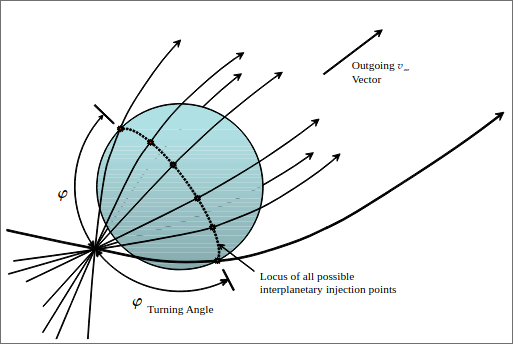
\includegraphics[width=\linewidth]{fig1.png}}
		\caption{Example Earth hyperbolic departure trajectories satisfying $v_{\infty}$. Image from Fundamentals of Astrodynamics and Applications \cite{b2}}
		\label{fig}
	\end{figure}
	
	The hyperbolic periapsis velocity and circular velocity can be solved as follows:
	\[
	\prescript{I(body)}{}{v_{circ}} = \sqrt{\frac{\mu_{body}}{r_{p(body)}}}
	\quad\text{,}\quad
	\prescript{I(body)}{}{v_{hp}} = \sqrt{v_{\infty}^2 + \frac{2\mu_{body}}{r_{p(body)}}}
	\]
	Subsequently,
	\[
	\Delta v_{body} = |\prescript{I(body)}{}{v_{hp}} - \prescript{I(body)}{}{v_{circ}}|
	\]
	This gives the delta-v to reach a circular orbit of $r_{p(body)}$ at each body based on the transfer orbit velocity at that body. Additional information, such as the time to get from body 1 to body 2 and the about the period of the transfer can be found:
	\[
	t_{transfer} = \pi \sqrt{\frac{a_{transfer}^3}{\mu_0}}
	\quad\text{,}\quad
	T_{syn} = (\frac{1}{T_{Earth}} - \frac{1}{T_{Mars}})^{-1}
	\]
	Where $T_{Earth}$ and $T_{Mars}$ are the orbital periods of Earth and Mars respectively.
	
	\subsection{Patched Conics Lambert Solution}
	Solving an interplanetary transfer using a Lambert solution follows essentially the same process, with two exceptions: the positions of the planets at departure and arrival must be known (typically they are found by pre-determining the time of flight), and the velocities at body 1 and body 2 are given by the Lambert solver. The variable $long$ specifies whether it will traverse  less than 180$^\circ$ about the central body, or more than 180$^\circ$.
	
	\[
	(\prescript{I0}{}{\vec{v}_1},\;\prescript{I0}{}{\vec{v}_2})
	= \mathrm{LambertSolver}\bigl(\prescript{I0}{}{\vec{R_1}},\;\prescript{I0}{}{\vec{R_2}},\;\mathrm{TOF},\;\mathrm{long}\bigr)
	\]
	
	With $\prescript{I0}{}{\vec{v}_1}$ and $\prescript{I0}{}{\vec{v}_2}$ in hand, the same patched conics solution as a Hohmann transfer can be applied to find $\Delta v$ at each body.
	
	Notably, unlike with a Hohmann transfer, the positions of the bodies can be determined by many different means. For example, one could have the bodies follow keplerian orbits about the sun and then estimate the positions at departure and arrival that way, or one could implement an n-body solver to determine the states of the bodies, and then pass the positions into a Lambert solver for a keplerian trajectory estimate in an n-body universe.
	
	\subsection{N-Body Simulation}
	
	Simulating the Solar System as an n-body system involves defining every body's standard gravitational parameters, and state vectors for t=0 (step 0). 
	
	\subsection{Application To Space Probe Design}
	
	With delta-v calculated, real-world mission analysis can begin. This involves two primary equations,
	\[
	\Delta v = I_{sp} \times g_0 \times ln\frac{m_i}{m_f}
	\quad\text{and}\quad
	m_{fuel} = m_i (1 - e^{\frac{-\Delta v}{I_{sp} g_0}})
	\]
	
	Where $m_i$ is the initial mass of the craft before the burn, and $m_f$ is the mass afterwards. $m_{fuel}$ represents the change in mass, or the amount of fuel burned.
	
	\section{Results}
	
	To compare the above two methods - simple Hohmann transfer and a patched-conics Lambert solution in an n-body solar system - a hypothetical mission to Mars with the following parameters is compared:
	\begin{itemize}
		\item Launch Inclination of 28.5$^\circ$ to 57$^\circ$ (CCSFS)
		\item Orbiter ($m_{wet}$ = 6300kg, $m_{dry}$ = 2300kg, with lander. $I_{sp}$ = 330s)
		\item Transfer Stage ($m_{wet}$ = 22825kg, $m_{dry}$ = 2326kg, not including payload. $I_{sp}$ = 465s)
	\end{itemize}
	
	With these initial values, the burn at Earth will have a wet and dry mass of $m_{wet} = 29125$ and $m_{dry} = 8626$, respectively. The burn at Mars will have the properties of the orbiter wet and dry mass. This yields available $\Delta v$ values of:
	\[
	\Delta v_{Earth} =465 \times 9.80665 \times ln\frac{29125}{8626} =  5.545 km/s
	\]
	\[
	\Delta v_{Mars} =330 \times 9.80665 \times ln\frac{6300}{2300} =  3.261 km/s
	\]
	
	\subsection{Simple Hohmann}
	The simple patched-conics Hohmann transfer between Earth and Mars yields a $\Delta v$ of $3.611km/s$ at Earth and $2.102km/s$ at Mars to exit/enter 180km parking orbits at both planets, with a time of flight of $258.840$ days. As $3.611km/s$ is less than the $5.545km/s$ available at Earth, and $2.102km/s$ is less than the $3.261km/s$ available at Mars, this transfer would allow a single impulsive burn by the transfer stage at Earth, followed by stage separation and a single impulsive burn at Mars for capture and circularization. Additionally, the synodic period was calculated as 2.136 years.
	
	\subsection{Lambert N-Body}
	To solve the Lambert problem, an N-body simulation was set up, with the t=0 epoch at April 1, 2025 12:00:00 UTC, and initial states of all planets and relevant moons captured from the NASA Horizons database. The states were then propogated using a Runge-Kutta 4th Order (RK4) numerical integrator, a common method for solving differential equations in orbital mechanics, computing steps three years ahead to April 1, 2027. The Lambert problem was iteratively solved for each possible departure step, with a range of travel time from 90 days to 360 days. The lowest delta-v Lambert solution was computed and displayed in a custom 3D graphical display.
	
	\begin{figure}[H]
		\centerline{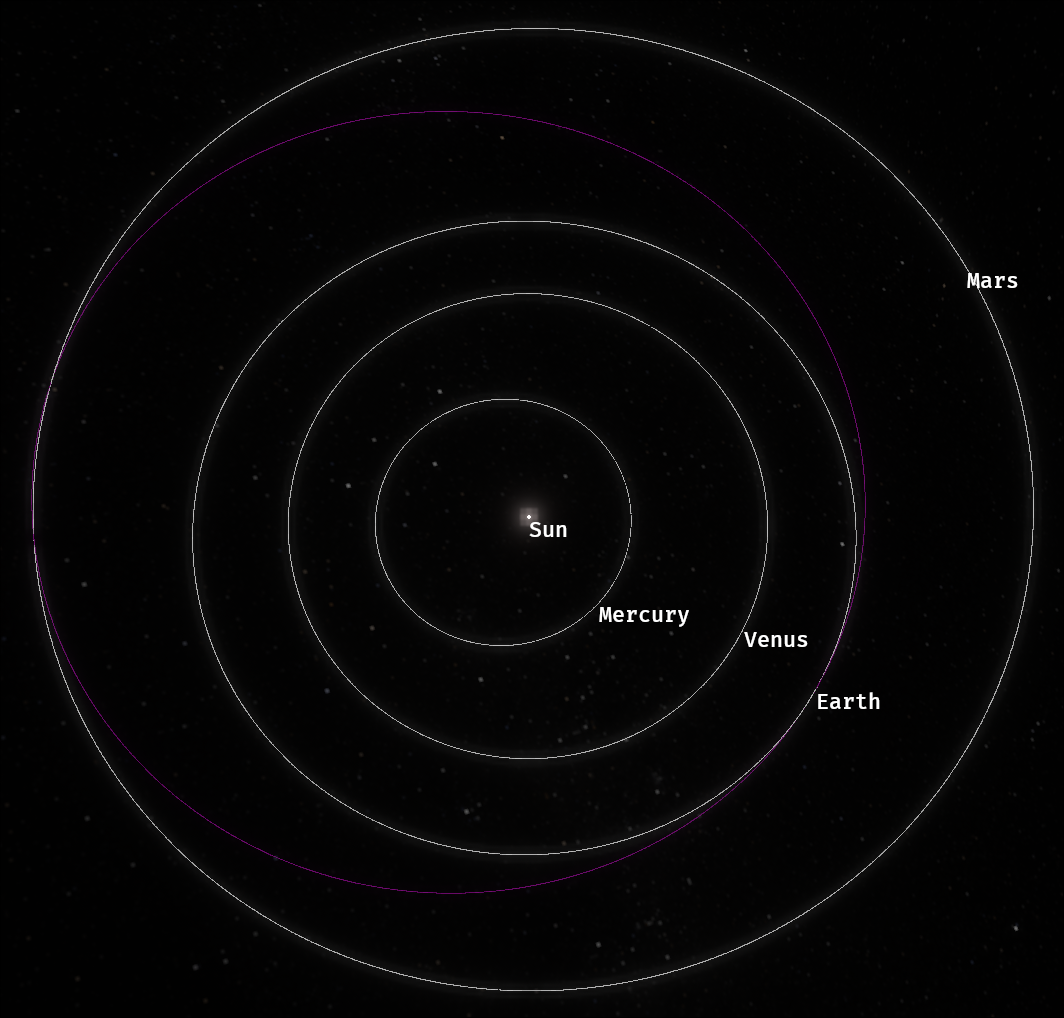
\includegraphics[width=\linewidth]{fig2.png}}
		\caption{Visualization of planetary positions and optimal transfer path (highlighted in purple) on 2026-10-31 in N-body simulation.}
		\label{fig2}
	\end{figure}
	
	After solving for the hyperbolic periapsis velocities at Earth and Mars, slightly different $\Delta v$ values emerge: $3.642km/s$ for Earth, and $2.065km/s$ for Mars. As $3.642km/s$ is less than the $5.545km/s$ available at Earth, and $2.065km/s$ is less than the $3.261km/s$ available at Mars, this transfer would allow a single impulsive burn by the transfer stage at Earth, followed by stage separation and a single impulsive burn at Mars for capture and circularization. It is worth noting that the delta-v requirement at Earth increases slightly; whereas the delta-v requirement at Mars decreased slightly. 
	
	\subsection{Comparison of Results}
	The simple Hohmann transfer in a patched-conics approximation, provides a simple and easy solution with a total $\Delta v$ requirement of approximately $5.713 km/s$ (sum of departure and arrival maneuvers). The transfer duration is fixed at 258.840 days, assuming circular, coplanar orbits. This approach is suitable for mission planning at a preliminary level, offering insight into baseline energy requirements and feasibility within propulsion limits.\\
	
	In contrast, the Lambert N-body solution incorporated the gravitational influence of multiple celestial bodies and non-Keplerian orbital perturbations. The iterative solution over thousands of departure dates and travel times (90–360 days) revealed a more optimized trajectory in terms of $\Delta v$. Particularly, it accounts for the real dynamics of the solar system, enabling a realistic trajectory plan. This method also accounts for actual eccentricities and inclinations of Earth and Mars, which are neglected in the simplified Hohmann model.\\
	
	In both situations, approximately $3.62km/s$ of delta-v is burned at Earth by the transfer stage, and $2.08km/s$ is burned by the orbiter at Mars to circularize.
	This means that, assuming that fuel in each craft is not reduced and there is no boiloff, the total mass burned will be as follows:
	\[
	Earth: m_{fuel} = 29125 (1 - e^{\frac{-3620}{465 * 9.80665}}) = 15957.5kg
	\]
	\[
	Mars: m_{fuel} = 6300 (1 - e^{\frac{-2080}{330 * 9.80665}}) = 2987.1kg
	\]
	
	It can be seen that the mission requirements are exceeded drastically, and both the orbiter and centaur could be launched with less fuel to save on costs. To further exceed $\Delta v$ requirements, the orbiter’s built-in ion engine - excluded from impulsive burn calculations - could be used post-capture to gradually lower apoapsis over time, possibly supplemented by aerobraking.
	
	\section{Conclusions and Future Work}
	
	In conclusion, a simple Hohmann transfer approximation provides a highly accurate $\Delta v$ estimate for an Earth-Mars transfer, although it is incapable of predicting the trajectory when accounting for eccentricity and inclination in the orbits. While the patched-conics Hohmann model offers an expedient baseline, integrating an N-body Lambert solution into mission planning bridges the gap between preliminary analysis and high-fidelity trajectory design. The marginal increase in Earth departure $\Delta v$ and corresponding decrease in Mars capture $\Delta v$ underscore the importance of realistic orbital geometry. This trade-off shows the need for iterative optimization in trajectory design to balance fuel efficiency with mission constraints and arrival conditions.
	
	\subsection{Future Work}
	
	With a baseline automatic trajectory designer implemented in an n-body solar system, there are two primary future developments would be both simple and helpful to implement: n-body iteration of the departure trajectory, and automatic iterative optimization of the departure burn to optimize arrival trajectory. While the departure trajectory provides a reliable hyperbolic trajectory which will roughly result in a Mars intersect, perturbation will inevitably result in some error, and even in an ideal patched conics universe, it would still not perfectly line up with the desired arrival hyperbola due to small changes in velocity.\\
	
	Additionally, after calculating all six orbital elements of the departure hyperbola which results in the correct $v_{\infty}$ which also satisfy launch inclination requirements, a model could be created to calculate the exact RAAN at which to begin the launch from CCSFS or another launch site, perhaps even taking into account J2 perturbation in reverse as a function of how long it is planned to be in the parking orbit. \\
	
	By iterating the Lambert solution, a porkchop plot was able to be generated, with the x-axis representing departure day (days since t=0 epoch), and the y-axis representing TOF. Although it would be very computationally expensive, an 'advanced' porkchop plot could hypothetically be generated, which could include potential benefits from gravity assists or other n-body interactions, revealing launch windows which would otherwise remain obscured. 
	
	\begin{figure}[H]
		\centerline{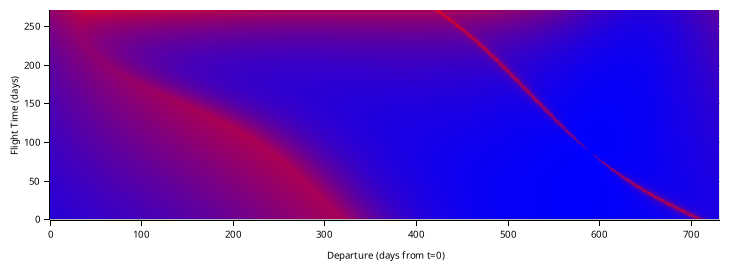
\includegraphics[width=\linewidth]{fig3.png}}
		\caption{Porkchop plot generated by iterating Lambert problem}
		\label{fig3}
	\end{figure}
	
	Another possible use of an n-body iterator is for non-impulsive burns. The iterator could be updated to include self-induced acceleration of a craft, with which more complex burns could be modeled and optimized by the n-body optimizer discussed previously.\\
	
	Another potential use of such a general purpose n-body optimizer would be targeted landings. It is likely that return flights from other planets (e.g. Mars Sample Return) would not want to enter a parking orbit of Earth before landing, likely preferring direct reentry. To target a specific landing site, a high fidelity n-body iterator would be required to perform very specific mid-course corrections on the return from Mars. An n-body iterator could perform this to target a specific landing site and angle of attack.
	
	\newpage
	
	\begin{thebibliography}{00}
			
			\bibitem{b1}
			L. M. Burke, R. D. Falck, and M. L. McGuire, “Interplanetary Mission Design Handbook: Earth‐to‐Mars Mission Opportunities 2026 to 2045,” NASA Technical Memorandum NASA/TM‐2010‐216764, Oct. 2010. [Online]. Available: https://ntrs.nasa.gov/api/citations/20100037210/downloads/20100037210.pdf
			\bibitem{b2}
			D. A. Vallado, \textit{Fundamentals of Astrodynamics and Applications}, 4th ed. Microcosm Press, 2013.
			\bibitem{b3}
			NASA STI Program Office, \textit{Interplanetary Mission Design Handbook}, NASA SP‐1998‐0015558, 1998. [Online]. Available: https://ntrs.nasa.gov/api/citations/19980210557/downloads/19980210557.pdf
			\bibitem{b4}
			M. Borges, “Revisiting the Dynamics of the Two‐Body Problem,” \textit{Mathematics}, vol. 12, no. 4, Art. 590, 2023. [Online]. Available: https://www.mdpi.com/2227-7390/12/4/590
			\bibitem{b5}
			“Two‐Body Problem,” ScienceDirect. [Online]. Available: https://www.sciencedirect.com/topics/earth-and-planetary-sciences/two-body-problem
			\bibitem{b6}
			R. J. Blassingame, “An Analysis of N‐Body Trajectory Propagation,” M.S. thesis, Dept. Aero. Eng., Cal Poly, San Luis Obispo, CA, 2011. [Online]. Available: https://digitalcommons.calpoly.edu/cgi/viewcontent.cgi?article=1049
			\bibitem{b9}
			“Patched Conic,” ScienceDirect. [Online]. Available: https://www.sciencedirect.com/topics/engineering/patched-conic
			\bibitem{b10}
			W. R. Hohmann, “The Law of Elliptical Orbit Transfers,” \textit{NASA TN D–2779}, Feb. 1960. [Online]. Available: https://ntrs.nasa.gov/citations/19690029384
			\bibitem{b11}
			J. H. Lambert, “Mémoire sur quelques propriétés remarquables des quantités transcendantes, circulaires et logarithmiques,” in \textit{Nouvelles Mémoires de l’Académie Impériale des Sciences de Berlin}, 1761.
			\bibitem{b12}
			Arizona State University, “Lecture 10: Rendezvous and Targeting – Lambert’s Problem,” 2023. [Online]. Available: https://control.asu.edu/Classes/MAE462/462Lecture10.pdf
			\bibitem{b13}
			C. G. Park, “Rapid Calculation of Spacecraft Trajectories Using Efficient Taylor Series Integration,” NASA Tech. Memo. NASA/TM‐2011‐216778, 2011. [Online]. Available: https://ntrs.nasa.gov/api/citations/20110003034/downloads/20110003034.pdf
			\bibitem{b14}
			Anonymous, “Numerical Integration in a Rigid‐Body Trajectory Program,” NASA Tech. Note D–4624, 1969. [Online]. Available: https://ntrs.nasa.gov/api/citations/19690029384/downloads/19690029384.pdf
			\bibitem{b15}
			J. P. Ludwig, “Mariner Mars 1964 Project Report,” NASA SP-65, Jet Propulsion Laboratory, Pasadena, CA, 1966. [Online]. Available: https://ntrs.nasa.gov/api/citations/19660021627/downloads/19660021627.pdf
			\bibitem{b16}
			A. K. Misra, “Trajectory Optimization for Planetary Missions: A Review,” \textit{Acta Astronautica}, vol. 181, pp. 642–655, 2021. [Online]. Available: https://doi.org/10.1016/j.actaastro.2020.12.020
	\end{thebibliography}
	
	\newpage
	
	\appendix
	\noindent\hfill
	\begin{minipage}{0.85\linewidth}
	\begin{lstlisting}[style=ieee-tight, caption={Hohmann Transfer Calculation MatLab}]
function [deltaV1, deltaV2, TOF] = hohmann_transfer(mu0, mu1, mu2, R1, R2, rp1, rp2)

	% heliocentric velocities
	v_circ1 = sqrt(mu0 / R1); 
	v_circ2 = sqrt(mu0 / R2); 
	
	a_trans = (R1 + R2) / 2; 
	
	v_trans1 = sqrt(mu0 * (2/R1 - 1/a_trans)); 
	v_trans2 = sqrt(mu0 * (2/R2 - 1/a_trans)); 
	
	% hyperbolic excess velocities
	v_inf1 = abs(v_trans1 - v_circ1); % at body1
	v_inf2 = abs(v_trans2 - v_circ2); % at body2
	
	% hyperbolic departure and arrival delta-v calculations
	v_esc1 = sqrt(v_inf1^2 + 2*mu1/rp1); 
	v_circ1_body = sqrt(mu1/rp1); 
	deltaV1 = v_esc1 - v_circ1_body;
	
	v_esc2 = sqrt(v_inf2^2 + 2*mu2/rp2);
	v_circ2_body = sqrt(mu2/rp2);
	deltaV2 = v_esc2 - v_circ2_body;
	
	%tof
	TOF = pi * sqrt(a_trans^3 / mu0);
	end
	
% Run the script for hohmann

% km^3 / s^2
mu0 = 1.327e11
mu1 = 3.986e5;  
mu2 = 4.282e4; 

R1 = 1.496e8;  
R2 = 2.279e8; 

rp1 = 6578;  
rp2 = 3594;  

[deltaV1, deltaV2, TOF] = hohmann_transfer(mu0, mu1, mu2, R1, R2, rp1, rp2);

fprintf('Delta-V at Body1 (departure): %.3f km/s\n', deltaV1);
fprintf('Delta-V at Body2 (arrival): %.3f km/s\n', deltaV2);
fprintf('TOF: %.3f days', TOF/86400);
	\end{lstlisting}
	\end{minipage}
	
\end{document}
